\documentclass[tocnosub,noragright,mixcasechap,centerchapter,12pt]{uiucecethesis09}

% Use draftthesis for notes and date markings on every page.  Useful when you
%   have multiple copies floating around.
% Use offcenter for the extra .5 inch on the left side. Needed with fullpage and fancy.
% Use mixcasechap for compatibility with hyperref package, which does NOT like all caps default
% Use edeposit for the adviser/committee on the title page.
% Use tocnosub to suppress subsection and lower entries in the TOC.
% PhD candidates use "proquest" for the proquest abstract.

\makeatletter

\usepackage{setspace}
\usepackage{epsfig}  % for figures
%\usepackage{graphicx}  % another package that works for figures
%\usepackage{subfigure}  % for subfigures
\usepackage{amsmath}  % for math spacing
%\usepackage{amssymb}  % for math spacing
%\usepackage{url}  % Hyphenation of URLs.
\usepackage{lscape}  % Useful for wide tables or figures.
\usepackage[justification=raggedright]{caption}	% makes captions ragged right - thanks to Bryce Lobdell
\usepackage{hyperref}
\hypersetup{
    colorlinks=true,
    linkcolor=blue,      
    urlcolor=cyan,
    citecolor=blue,
}

\usepackage{amsmath}
\usepackage{multirow}
\usepackage{multicol}
\usepackage{colortbl}
\usepackage{xspace}
\usepackage{graphicx}
\usepackage{booktabs}
\usepackage{algorithm2e}
\usepackage{circledsteps}
\usepackage{amsmath}
\usepackage{amssymb}

\newcommand{\TODO}[1]{\textcolor{red}{TODO: #1}}
\newcommand{\original}[1]{\textcolor{brown}{#1}}
\newcommand{\perturbed}[1]{\textcolor{teal}{#1}}
\newcommand{\correct}[1]{\textcolor{teal}{#1}}
\newcommand{\wrong}[1]{\textcolor{purple}{#1}}
\newcommand{\correcteq}{$\textcolor{teal}{\checkmark}$}
\newcommand{\wrongeq}{$\textcolor{purple}{\times}$}
\newcommand{\tabincell}[2]{\begin{tabular}{@{}#1@{}}#2\end{tabular}}
\newcommand{\perfdrop}[2]{#1\% absolute drop and #2\% relative drop}
\newcommand{\perfimprove}[2]{#1\% absolute improvement and #2\% relative improvement}

\newcommand{\refequ}[1]{Equation~(\ref{#1})}
\newcommand{\reffig}[1]{Figure~\ref{#1}}
\newcommand{\refsec}[1]{\S\ref{#1}} % \textsection
\newcommand{\reftab}[1]{Table~\ref{#1}}
\newcommand{\refdef}[1]{Definition~\ref{#1}}
\newcommand{\refalgo}[1]{Algorithm~\ref{#1}}
\newcommand{\refapp}[1]{Appendix~\ref{#1}}


\def\eg{\textit{e.g.}\xspace}
\def\Eg{\textit{E.g.}\xspace}
\def\etal{\textit{et al.}\xspace}
\def\etc{\textit{etc.}\xspace}
\def\ie{\textit{i.e.}\xspace}
\def\Ie{\textit{I.e.}\xspace}
\def\vs{\textit{vs.}\xspace}
\def\wrt{\textit{w.r.t.}\xspace}


% Uncomment the appropriate one of the following four lines:
\bsthesis
%\phdthesis
%\otherdoctorate[abbrev]{Title of Degree}
%\othermasters[abbrev]{Title of Degree}

\title{GENERATIVE CONTRASTIVE LEARNING FOR~STRUCTURAL~FRAMING~ANALYSIS}
\author{Jialiang Xu}
\department{Electrical and Computer Engineering}
\degreeyear{2022}

% Advisor name is required for
% - doctoral students for the ProQuest abstract
% - master's students who do not have a master's committee
\advisor{Heng Ji}

% Uncomment the \committee command for
% - all doctoral students
% - master's students who have a master's committee
%\committee{Professor Firstname Lastname, Chair\\
%        Professor Firstname Lastname} % etc.

\begin{document}

%%%%%%%%%%%%%%%%%%%%%%%%%%%%%%%%%%%%%%%%%%%%%%%%%%%%%%%%%%%%%%%%%%%%%%%%%%%%%%%
% COPYRIGHT
%
%\copyrightpage
%\blankpage

%%%%%%%%%%%%%%%%%%%%%%%%%%%%%%%%%%%%%%%%%%%%%%%%%%%%%%%%%%%%%%%%%%%%%%%%%%%%%%%
% TITLE
%
\maketitle

%\raggedright
\parindent 1em%

\frontmatter

%%%%%%%%%%%%%%%%%%%%%%%%%%%%%%%%%%%%%%%%%%%%%%%%%%%%%%%%%%%%%%%%%%%%%%%%%%%%%%%
% ABSTRACT
%
\begin{abstract}
% Put the abstract in a file called "abs.tex" and it'll be inputted here.
Framing is the act ``to select some aspects of a perceived reality and make them more salient in a communicating text'' \cite{entman1993}. Framing has been widely used in journalism to influence public opinion. However, analysis of news framing has majorly relied on human expert efforts. Efforts have been put into developing automatic framing analysis via computational linguistic approaches. In this paper, we propose a novel large-scale, multi-agency news dataset with crowd-sourced political stances and factuality labels to facilitate framing analysis. We propose two ways of conducting framing analyses on this dataset, the first is via learning a ``switch'' in the embedding space to change the generation trend, and the second utilizes a Generative Adversarial Network under a contrastive learning framework. We further create an interactive demo website to directly display results. Our code and dataset will be released to facilitate future research.
\end{abstract}


%%%%%%%%%%%%%%%%%%%%%%%%%%%%%%%%%%%%%%%%%%%%%%%%%%%%%%%%%%%%%%%%%%%%%%%%%%%%%%%
% DEDICATION
%
\begin{dedication}
% Whatever dedication you want.
To my parents, for their love and support.
\end{dedication}

%%%%%%%%%%%%%%%%%%%%%%%%%%%%%%%%%%%%%%%%%%%%%%%%%%%%%%%%%%%%%%%%%%%%%%%%%%%%%%%
% ACKNOWLEDGMENTS
%
% Put acknowledgments in a file called "ack.tex" and it'll be inputted here.
\begin{acknowledgments}
This endeavor would not have been possible without my research advisor Prof. Heng Ji and her priceless feedback and inspiration. She has been the perfect advisor, providing more support and guidance than I ever ask for. 

I also could not have undertaken this journey without my mentors Manling Li and Chi Han, who generously helped me with their extraordinary knowledge and experience. Cooperating with them has been one of the most rewarding experiences of mine.

I am also grateful to my family and friends, for their belief in me has helped me stay motivated throughout this process. I would also like to thank my Syrian hamster, Jeremy, for all of the entertainment and emotional support.
\end{acknowledgments}

%%%%%%%%%%%%%%%%%%%%%%%%%%%%%%%%%%%%%%%%%%%%%%%%%%%%%%%%%%%%%%%%%%%%%%%%%%%%%%%
% TABLE OF CONTENTS
%
\tableofcontents

%%%%%%%%%%%%%%%%%%%%%%%%%%%%%%%%%%%%%%%%%%%%%%%%%%%%%%%%%%%%%%%%%%%%%%%%%%%%%%%
% LIST OF TABLES
%
% The List of Tables is not strictly necessary. Omitting the List of Tables will
% simplify the thesis check and reduce the number of corrections.
% \listoftables

%%%%%%%%%%%%%%%%%%%%%%%%%%%%%%%%%%%%%%%%%%%%%%%%%%%%%%%%%%%%%%%%%%%%%%%%%%%%%%%
% LIST OF FIGURES
%
% The List of Figures is not strictly necessary. Omitting the List of Figures will
% simplify the thesis check and reduce the number of corrections.
% \listoffigures

%%%%%%%%%%%%%%%%%%%%%%%%%%%%%%%%%%%%%%%%%%%%%%%%%%%%%%%%%%%%%%%%%%%%%%%%%%%%%%%
% LIST OF ABBREVIATIONS
%
% The List of Abbreviations is not strictly necessary.
% \chapter{LIST OF ABBREVIATIONS}

%\begin{symbollist*}
%\item[EPIC] Explicitly Parallel Instruction Computing
%\item[GPU] Graphics Processing Unit
%\item[VLIW] Very Long Instruction Word
%\end{symbollist*}


%%%%%%%%%%%%%%%%%%%%%%%%%%%%%%%%%%%%%%%%%%%%%%%%%%%%%%%%%%%%%%%%%%%%%%%%%%%%%%%
% LIST OF SYMBOLS
%
%\begin{symbollist}[0.7in]
%\item[$\tau$] Time taken to drink one cup of coffee.
%\end{symbollist}

\mainmatter

%%%%%%%%%%%%%%%%%%%%%%%%%%%%%%%%%%%%%%%%%%%%%%%%%%%%%%%%%%%%%%%%%%%%%%%%%%%%%%%
% INSERT REAL CONTENT HERE
%

\chapter{Introduction}

News is an important medium through which the members of society get to understand the world. However, despite the normative expectation of neutrality and objectivity \cite{schudson2001objectivity}, news articles covering the same event can vary among different news agencies. The same story can be covered from different perspectives, conventionally referred to as ``frames'' \cite{entman1993,entman2007,entman2010media}. The act ``to frame'' is ``to select some aspects of a perceived reality and make them more salient in a communicating text'' \cite{entman1993}. As a linguistic technique, the practice of framing reflects the underlying preferences and intents of the covering news agency and is known to affect public opinion and political processes \cite{chong2007framing,iyengar1990framing,mccombs2002agenda,price2005framing,rugg1941experiments,schuldt2011global,baumgartner2008decline,dardis2008media,hamborg2020media,drakulich2015explicit,sap2019social}.

Prior work has proposed computational approaches for news framing analysis. One line of work focuses on recovering the underlying bias of the news agencies (\ie, Political Viewpoint Identification) \cite{PVI-survey,li-goldwasser-2021-using,kim-johnson-2022-close,matero-etal-2021-melt-message,li-caragea-2021-multi}, and another line of work aims to locate the framing language and structures in the news articles \cite{hamborg2020media,drakulich2015explicit,sap2019social,baumer-etal-2015-testing}. Recently, there are also efforts paid to generate texts with framing techniques, such as the task of reframing \cite{ziems-etal-2022-inducing,chen-etal-2021-controlled-neural}.

In this work, we propose \texttt{MultiAgencyNews}, a novel large-scale, multi-agency news dataset with crowd-sourced political stances and factuality labels to facilitate framing analysis. Existing news aggregation platforms are utilized to collect metadata for recent social events with news article coverage from multiple news agencies. The metadata includes a series of labels including the news article URLs, news agency names, news agency political stance biases, and news agency factualities. The news articles are filtered with heuristics to balance the labels, guaranteeing that the comparison is fairly conducted.

We continue to propose two different methods of conducting framing analyses on this dataset, the first method, \texttt{SwitchLM}, learns a ``switch'' in a large pre-trained language model's embedding space, the switch shifts the semantic embedding of specific words in a text prompt for text generation. The switch is a learnable parameterized matrix that projects embedding for each word to a linear subspace, where the semantics of corresponding dimensions align with the corresponding directions in a scaled manner.

The second method, \texttt{GenCo}, utilizes generative language models and contrastive learning. An initial configuration vector is inputted to a generator, which is a generative language model such as \texttt{T5}, \texttt{BART}, and \texttt{GPT}. Existing Information Extraction tools are then applied to extract the event structure of the generated news, where two levels of event graphs are involved: 1) the inter-subframe graphs which capture the coarse-grained semantics such as paragraphs, and 2) the intra-subframe graphs which capture the fine-grained semantics such as sentences. The generated event graph is then compared with texts sampled from corresponding news pools from the dataset for contrastive learning with a classifier. The generator and the classifier are collectively trained and mutually enhancing each other.

We further create an interactive demo application with streamlit to directly display results. The application is live and hosted on a cloud server which can be accessed with public IP. The application showcases two functionalities: 1) the \textit{stance-guided generation} functionality, where the user gets to specify a stance on a continuous spectrum which will be used to guide the model on generating with stances, and 2) the \textit{text stance scoring} functionality, where a user-specified piece of news article text can be inferred by a hosted trained model to profile the underlying political bias.
\chapter{Related Works}

Previous relevant works have been focused on computational approaches of Political Viewpoint Indentification, framing mechanism, and the steerability of generative models.

\section{Political Viewpoint Indentification}
A line of work has been focused on automatic news framing analysis such as Political Viewpoint Identification (PVI) \cite{PVI-survey,li-goldwasser-2021-using,kim-johnson-2022-close,matero-etal-2021-melt-message,li-caragea-2021-multi,yu2008classify,hoyland-etal-2014-predicting,biessmann2016pvi,duthie2016mining,baly-etal-2019-multi,li2017pvi-lstm,rao2016pvi-lstm,gangula-etal-2019-detecting,kummervold-etal-2021-operationalizing,baly-etal-2020-detect,luo-etal-2020-detecting}. The task of PVI is to infer the political stance of the writer news agency from the news article content under a classification setting. Earlier work with traditional feature engineering techniques utilizes features such as tf-idf \cite{yu2008classify}, bag-of-words \cite{yu2008classify,hoyland-etal-2014-predicting,biessmann2016pvi}, and part-of-speech tags \cite{hoyland-etal-2014-predicting,duthie2016mining,baly-etal-2019-multi}.

More recent work has put more effort to leverage the success of deep learning language models and techniques, with a variety of backbones ranging from LSTM and its variations \cite{li2017pvi-lstm,rao2016pvi-lstm,gangula-etal-2019-detecting} to transformer-based models \cite{kummervold-etal-2021-operationalizing,baly-etal-2020-detect,luo-etal-2020-detecting}. This line of work relies more on word embedding and attention to capture the semantics behind news article contents.


\section{Framing Mechanism}
Another relevant domain is the analysis of the mechanism of framing. Earlier efforts have explored the task of framing language identification \cite{hamborg2020media,drakulich2015explicit,sap2019social,baumer-etal-2015-testing}. This task mainly aims to conduct word-level binary classification for framing languages. However, this effort is subject to the elusive nature of the framing language and has difficulty in obtaining high-quality annotation.

Another recent line of work focuses more on understanding the framing strategies used \cite{field-etal-2018-framing,ziems-yang-2021-protect-serve} and using the framing strategies for generation, with specific targets such as positive reframing \cite{ziems-etal-2022-inducing} and controlled reframing \cite{chen-etal-2021-controlled-neural}. 

Correspondingly, there have emerged open tools \cite{bhatia-etal-2021-openframing} to facilitate framing analysis for non-experts in computer science.

\section{Steerability of Generative Models}
Our method \texttt{SwitchLM} navigates the generative language models via learning a  projection matrix in the word embedding space. This technique has been previously applied to visual edition \cite{jahanian2019steerability,denton2019facial,shen2019facial,goetschalckx2019visual} to learn editing operations as linear trajectories in the latent space of Generative Adversarial Networks. 

Previous applications include image dimension editing \cite{jahanian2019steerability} where the output image can be parallelly or circularly shifted, facial feature finetuning and augmenting \cite{denton2019facial,shen2019facial} where the facial features can be finetuned or perturbed, and cognitive property transformation \cite{goetschalckx2019visual} where dimensions such as memorability, aesthetics, and emotional valence are altered.
\chapter{Methodology}

This is the Methodology part of the paper.
\chapter{Empirical Study and Analysis}
We provide more empirical study results on the \texttt{MultiAgencyNews} dataset by comparing news articles from left- and right-wing news agencies. We present a word cloud visualization of the news article contents in \refsec{empirical-wordcloud}, a topic modeling visualization with LDA in \refsec{empirical-lda}, an AMR graph visualization in \refsec{empirical-amr}, and a PVI baseline with a BERT backbone in \refsec{empirical-bert-pvi}. 

For the word cloud, LDA visualization, and AMR visualization, the topic of their corpus is gun control\footnote{\url{https://ground.news/interest/gun-control}}. For the BERT PVI baseline, the whole dataset is used.

\section{Word Cloud by Frequency}
\label{empirical-wordcloud}
The news article content of a gun control news\footnote{\url{https://tinyurl.com/2nzw6c3m}} is modeled with word cloud\footnote{\url{https://pypi.org/project/wordcloud/}} and shown in \reffig{fig:empirical-wordcloud-left}. On the Left side, the discussion is inclined towards the assault weapons themselves and their consequences, while on the Right side discussion is inclined towards the bill itself, the opponents' partisanship, and political concepts.

\begin{figure}[ht]
    \centering
    \begin{minipage}[b]{0.45\textwidth}
        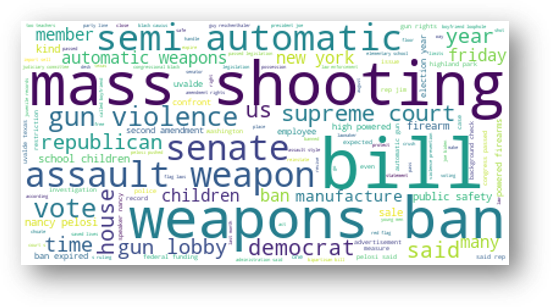
\includegraphics[width=\textwidth]{img/empirical-wordcloud-left}
        \caption{Wordcloud of Left-wing News Articles.}
        \label{fig:empirical-wordcloud-left}
    \end{minipage}
    \hfill
    \begin{minipage}[b]{0.45\textwidth}
        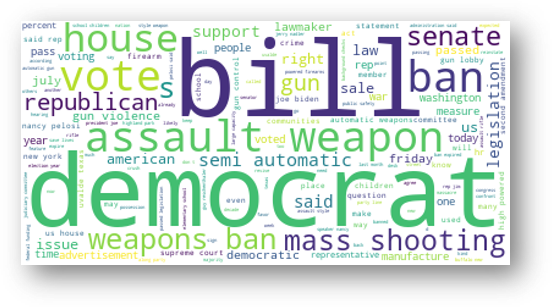
\includegraphics[width=\textwidth]{img/empirical-wordcloud-right}
        \caption{Wordcloud of Right-wing News Articles.}
        \label{fig:empirical-wordcloud-right}
    \end{minipage}
\end{figure}

\section{Topic Modeling with LDA}
\label{empirical-lda}
We also apply Latent Dirichlet Allocation (LDA) topic modeling on the dataset to compare the topics on both sides. The results are shown in \reffig{fig:empirical-lda-left} and \reffig{fig:empirical-lda-right}. On the Left side, topics are more dispersed, and the discussion on the ban itself is equivalent to weapons, while on the Right side topics are more focused, and the largest topic emphasizes the ban itself more than the weapons.

\begin{figure}[ht]
    \centering
    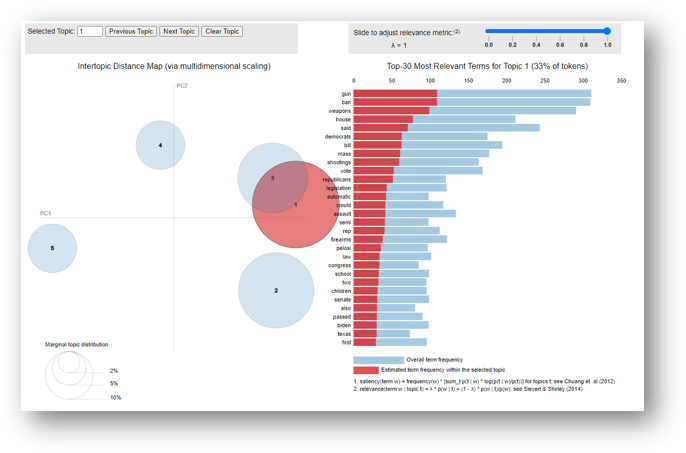
\includegraphics[width=0.8\textwidth]{img/empirical-lda-left}
    \caption{LDA Topic Modelling Result of Left-wing News Articles.}
    \label{fig:empirical-lda-left}
\end{figure}
\begin{figure}[ht]
    \centering
    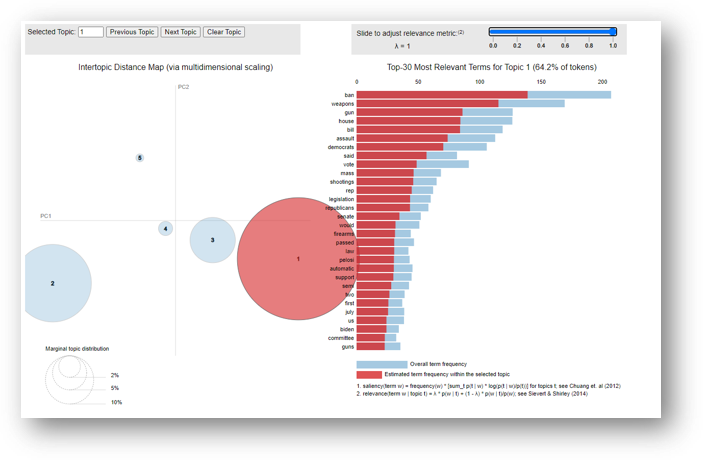
\includegraphics[width=0.8\textwidth]{img/empirical-lda-right}
    \caption{LDA Topic Modelling Result of Right-wing News Articles.}
    \label{fig:empirical-lda-right}
\end{figure}

\section{AMR Graph Modeling}
\label{empirical-amr}
The Abstract Meaning Representation (AMR) graphs are also extracted to compare the article structures on both sides. The results are shown in \reffig{fig:empirical-amr-left} and \reffig{fig:empirical-amr-right}. In addition to the basic facts (shooter age, place of incident, \etc), the news article on the Left side pointed out the emotions (``sad'' / ``anger''), while the news article on the Right side emphasizes the critical injury to the officer (``situation'' / ``critical'').

\begin{figure}[ht]
    \centering
    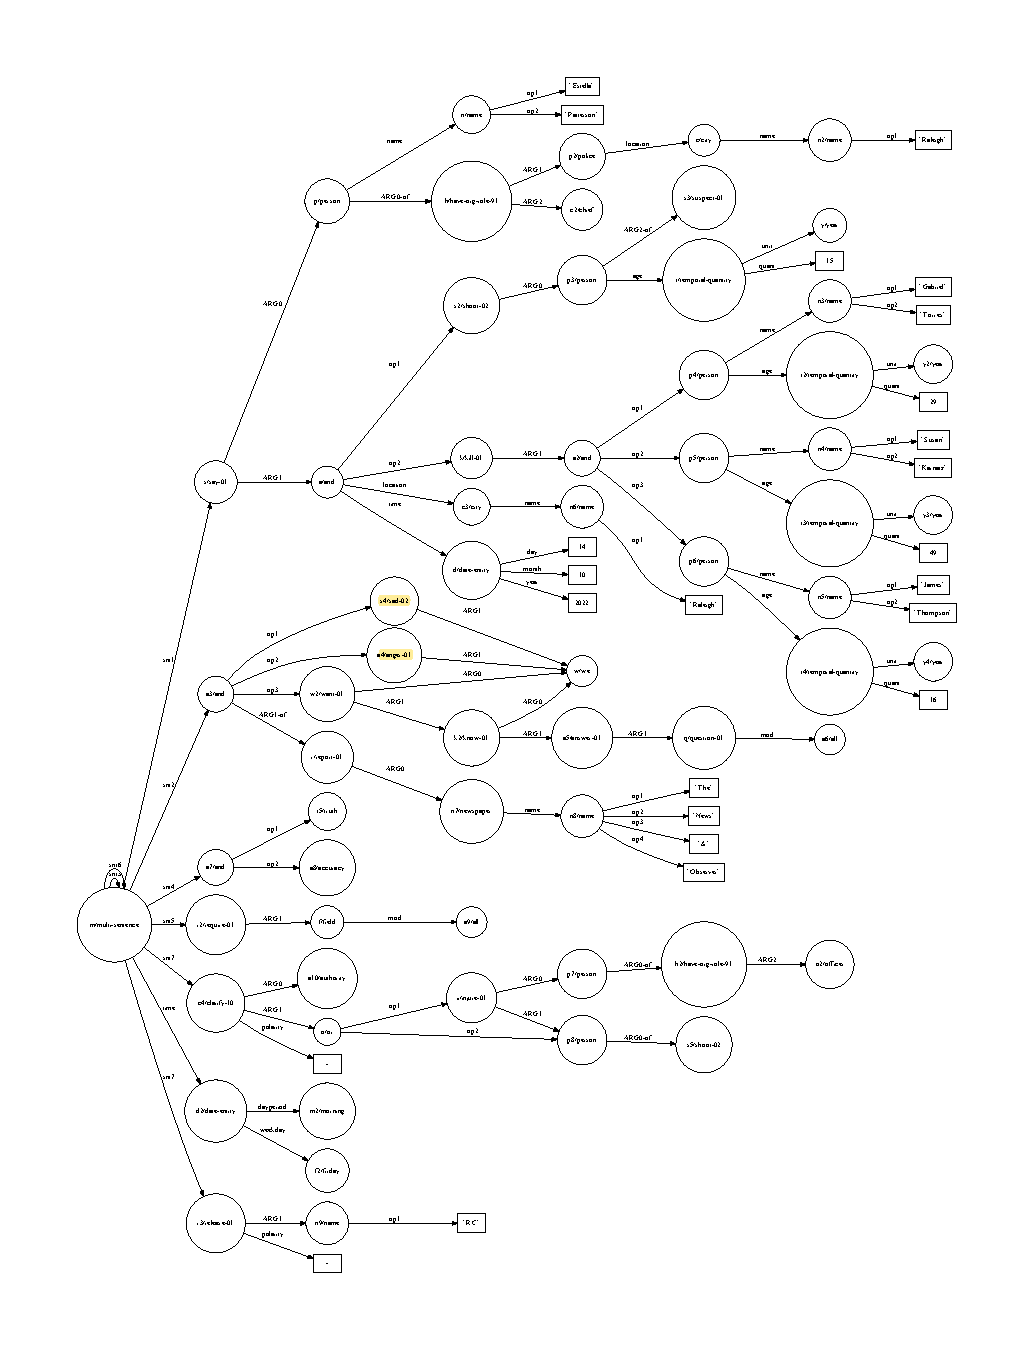
\includegraphics[width=0.9\textwidth]{img/empirical-amr-left}
    \caption{The AMR Graph of Left-wing News Articles.}
    \label{fig:empirical-amr-left}
\end{figure}
\begin{figure}[ht]
    \centering
    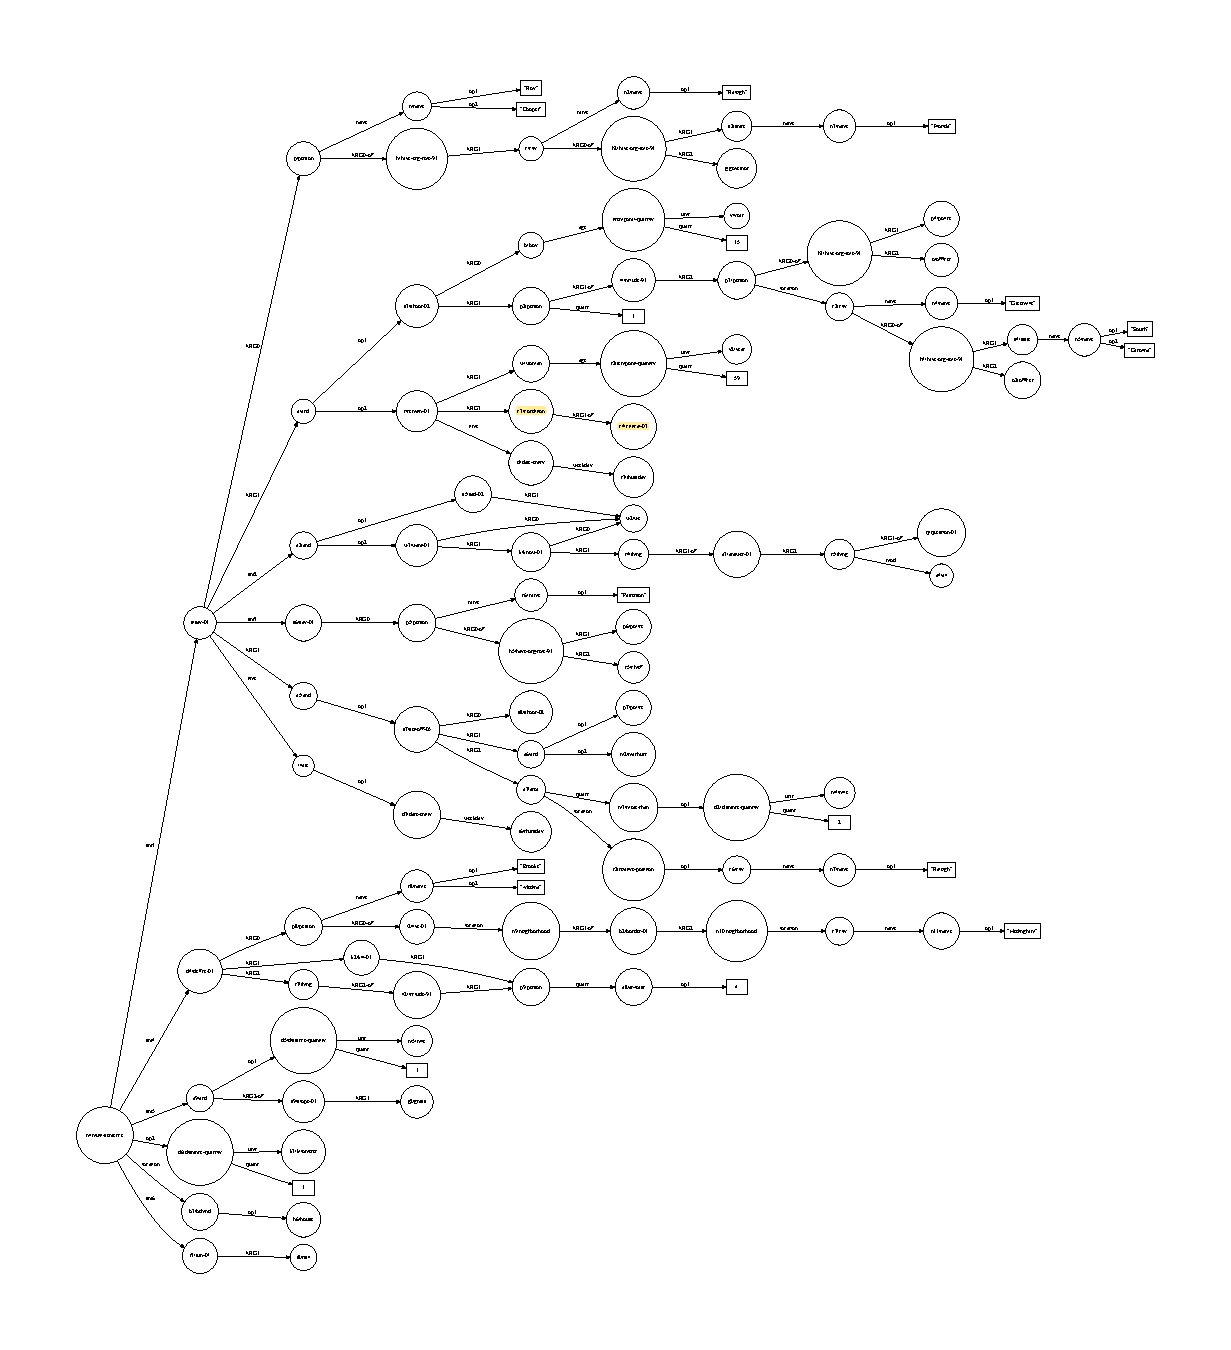
\includegraphics[width=\textwidth]{img/empirical-amr-right}
    \caption{The AMR Graph of Right-wing News Articles.}
    \label{fig:empirical-amr-right}
\end{figure}
\clearpage

\section{BERT PVI Baseline}
\label{empirical-bert-pvi}
To evaluate how challenging the dataset is for Political Viewpoint Identification (PVI), we finetuned a BERT model for sequence classification. The finetuning started with a vanilla bert-base-uncased checkpoint from HuggingFace Transformers\footnote{\url{https://huggingface.co/bert-base-uncased}}. The task is formulated as a 2-way classification with binary cross entropy loss. The dataset was split into training, validation, and test sets at the ratio of 0.7/0.1/0.2. The results are shown in \reffig{fig:empirical-bert-baseline}. The baseline model achieved only 59.19\% accuracy on the test set, which is only marginally higher than random guessing. This implies that PVI on the \texttt{MultiAgencyNews} dataset is still a challenging task.

\begin{figure}[ht]
    \centering
    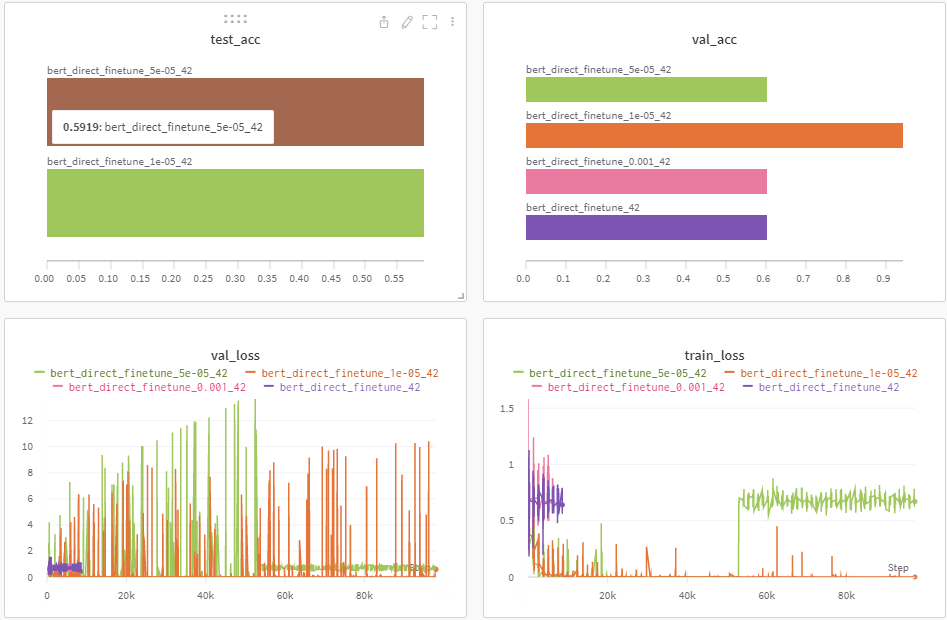
\includegraphics[width=\textwidth]{img/empirical-bert-baseline}
    \caption{The AMR Graph of Left-wing News Articles.}
    \label{fig:empirical-bert-baseline}
\end{figure}

\chapter{Interactive Demo Application}
We designed and implemented an interactive demo application\footnote{\url{http://switch.blenderdemo.com:8501/}} hosted on an AWS Cloud server to demonstrate our framing analysis functionalities. The demo application is based on Streamlit\footnote{\url{https://streamlit.io/}}. In the following sections, we elaborate on two functionalities of the demo application: 1) Text generation controlled by user-specified left-right stance position in \refsec{demo-generation}, and 2) Left-right stance categorization given text input in \refsec{demo-detection}.


\section{Stance-guided Generation}
\label{demo-generation}
A screenshot of the interface for Stance-guided Generation is shown in \reffig{fig:demo-generation}. A continuous slide bar controls the left-right position of text generation, and the user can specify the random seed and the max/min generation length for more generation control. The user can then input prefix text for the model to continue writing. After the ``Generate!'' button is clicked, the generated text will be displayed.


\begin{figure}[ht]
    \centering
    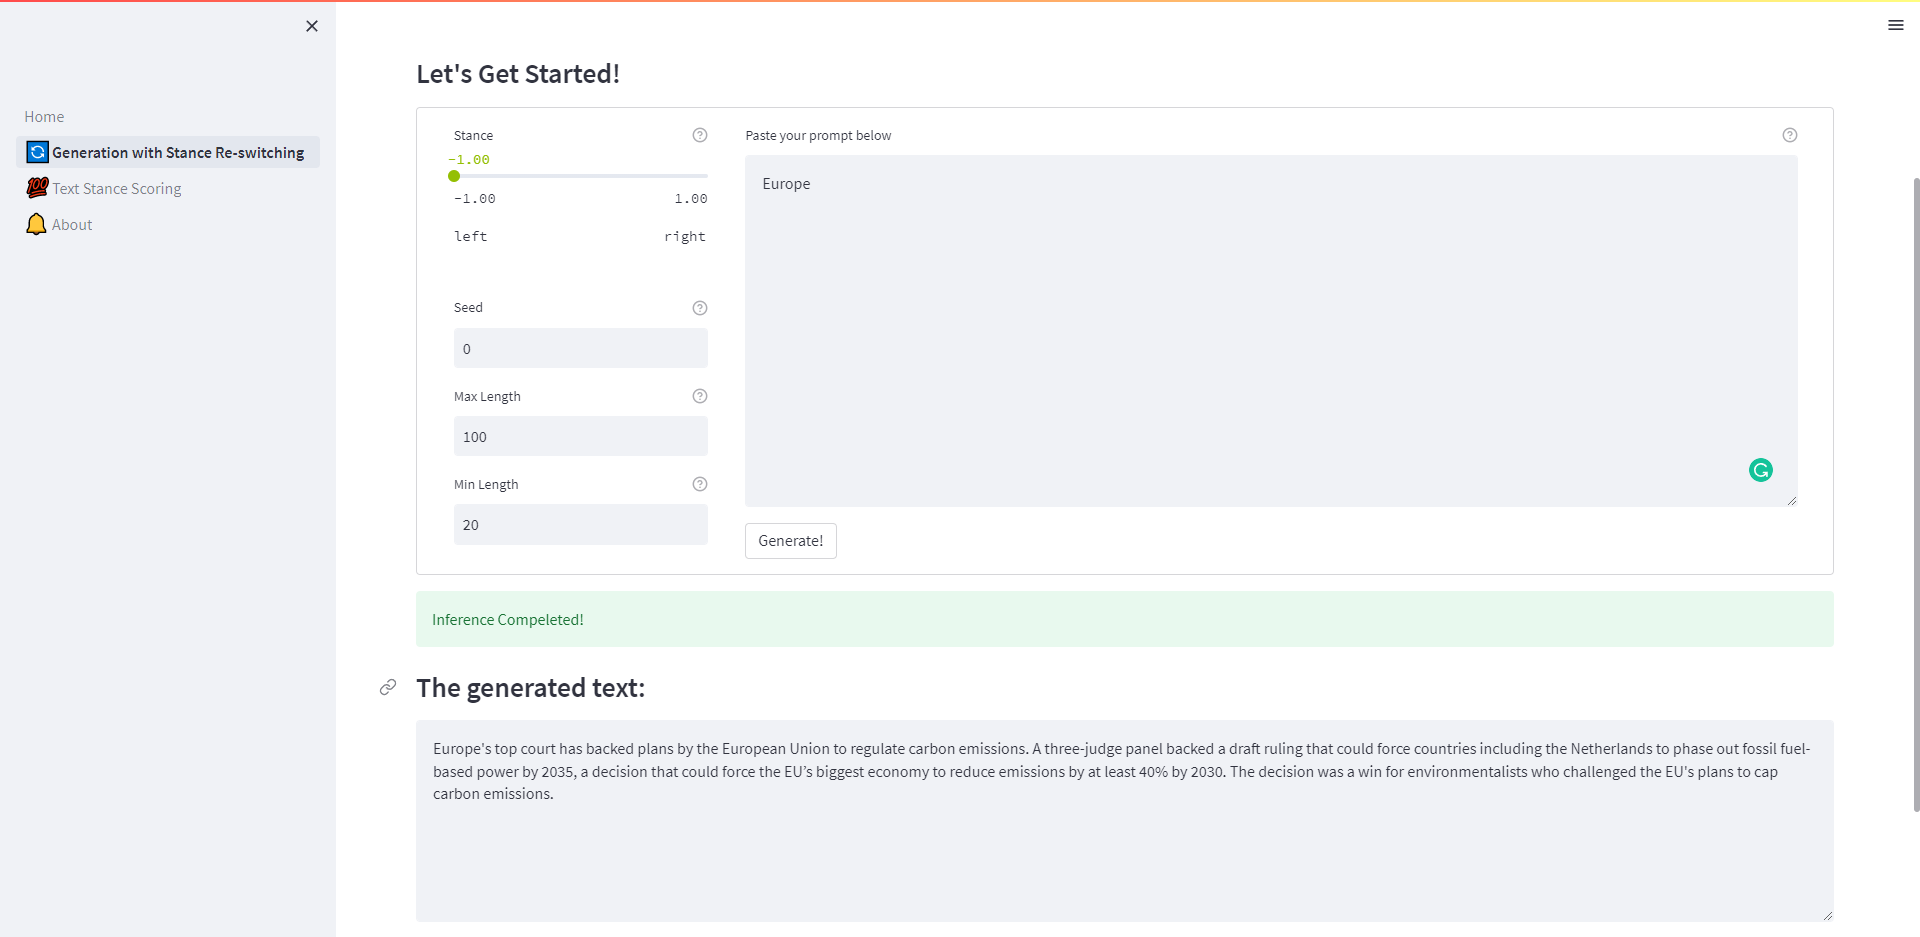
\includegraphics[width=\textwidth]{img/demo-generation}
    \caption{The interface of the Stance-guided Generation functionality.}
    \label{fig:demo-generation}
\end{figure}


\section{Stance Categorization}
\label{demo-detection}
A screenshot of the interface for Stance Categorization is shown in \reffig{fig:demo-detection}. An input box allows the user to put in the text to be analyzed. After clicking on the ``Analyze!'' button, two results will be output and displayed: 1) distribution of the probability across all 7 different stance categories, in the form of a histogram chart, and 2) a list-out of text spans that serve as evidence for the stance categorization and their evidence scores.


\begin{figure}[ht]
    \centering
    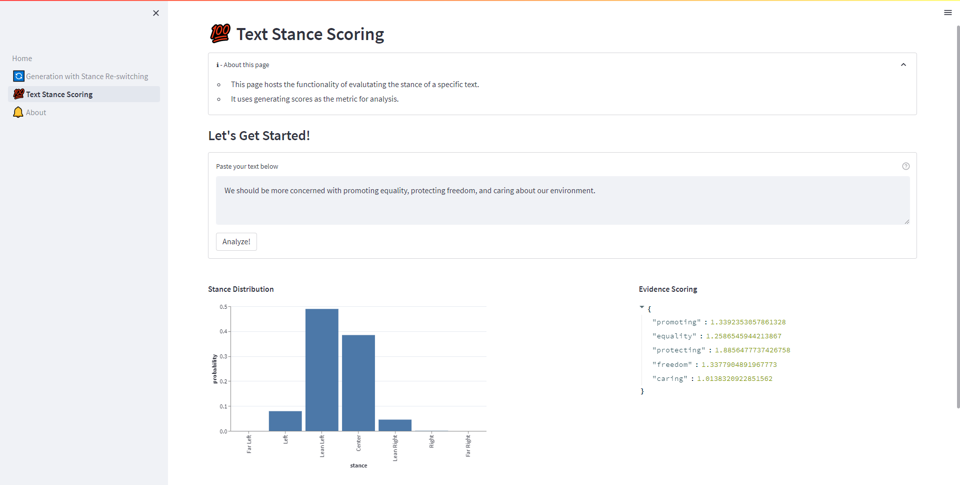
\includegraphics[width=\textwidth]{img/demo-detection}
    \caption{The interface of the Stance Categorization functionality.}
    \label{fig:demo-detection}
\end{figure}
\chapter{Conclusion}
In this paper, we propose a novel large-scale, multi-agency news dataset with crowd-sourced political stances and factuality labels to facilitate framing analysis. To conduct framing analysis on this dataset, two methods are proposed. The first is via learning a ``switch'' in the embedding space to latently edit the word embeddings, and the second utilizes a generative contrastive learning framework. We further conduct empirical studies and analysis to compare the news article differences from both political stances sides. We create an interactive demo website to directly display our pipelines.


%%%%%%%%%%%%%%%%%%%%%%%%%%%%%%%%%%%%%%%%%%%%%%%%%%%%%%%%%%%%%%%%%%%%%%%%%%%%%%%
% APPENDIX
%
% \appendix
% \chapter{Hierarchy of the \texttt{Ground.News} Website}


\backmatter

%%%%%%%%%%%%%%%%%%%%%%%%%%%%%%%%%%%%%%%%%%%%%%%%%%%%%%%%%%%%%%%%%%%%%%%%%%%%%%%
% BIBLIOGRAPHY
%
\bibliographystyle{IEEE_ECE}
% Put references in BibTeX format in thesisrefs.bib.
\bibliography{thesisrefs, anthology}


%%%%%%%%%%%%%%%%%%%%%%%%%%%%%%%%%%%%%%%%%%%%%%%%%%%%%%%%%%%%%%%%%%%%%%%%%%%%%%%
% AUTHOR'S BIOGRAPHY
% As of 10/03/2011, Author's Biography or Vita no longer accepted by Grad College

\end{document}
\endinput
